To implement the proposed architecture, first, the \gls{rpi} was loaded with a 
headless distribution of the Raspbian \citep{raspbian_raspbian_2018} operating system. 
Raspbian is a specialised GNU/Linux distribution based on Debian, optimized for 
the \gls{rpi}. 
It comes with over 35,000 packages including the Python programming language. 
Python will be used to create and run the script that comprises the implementation
of the client side system.
After setting up the \gls{rpi} and connecting the DHT22 sensor to the \gls{rpi}'s
\gls{gpio} pins as per \figref{fig:rpi_wiring}, a Python script was constructed
to collect the sensor data and, using \gls{coap}, send the data to the ThingsBoard
\citep{thingsboard_inc._thingsboard_2018} endpoint. 

The \gls{coap} client is created using the Python package, CoAPthon
\citep{tanganelli_coapthon3_2018}. 
This package contains a \texttt{HelperClient} class that takes a \gls{coap} 
path and port upon initialisation. 
An object is created using the path to the 
ThingsBoard telemetry endpoint and the default \gls{coap} port of 5683.
This \gls{coap} client object will be used to send the POST message containing
the data to the ThingsBoard cloud.

To retrieve the readings from the DHT22 sensor,
first, the Adafruit DHT22 library \citep{adafruit_adafruit_python_dht_2018} 
was imported to the script. This library contains a \texttt{read\_retry()} 
method that will attempt to read the temperature and humidity data from the 
DHT22 sensor and return values as floating point decimals; 
if no reading is available it will try again up to a specified number of retries,
defaulting to fifteen.

\begin{listing}[H]
    \begin{minted}
        [fontsize=\footnotesize,linenos,escapeinside=||,tabsize=2,breaklines]
        {js}
        {
            'temperature': 22.6,
            'humidity': 30.05
        }
    \end{minted}
    \caption{Sensor data formatted to \gls{json} for message payload.}
    \label{lst:payload_format}
\end{listing}

Once the sensor data is returned, the payload is constructed. The payload 
consists of the temperature and humidity data formatted into a JSON object, 
shown in \lstref{lst:payload_format}. This data is converted using the built-in
Python \gls{json} library. 
With the formatted payload, the \gls{coap} message is sent to the ThingsBoard
endpoint; the responding message from the ThingsBoard node is printed to the console.
Here, the script will wait a specified amount of time and then will repeat the 
process from retrieving the data. This process is shown in 
\algref{alg:get_send_data_alg}. 
% The Python script that accomplishes this is shown in the \hyperref[app:A]{Appendix}.

\begin{figure}[H]
    \centering
    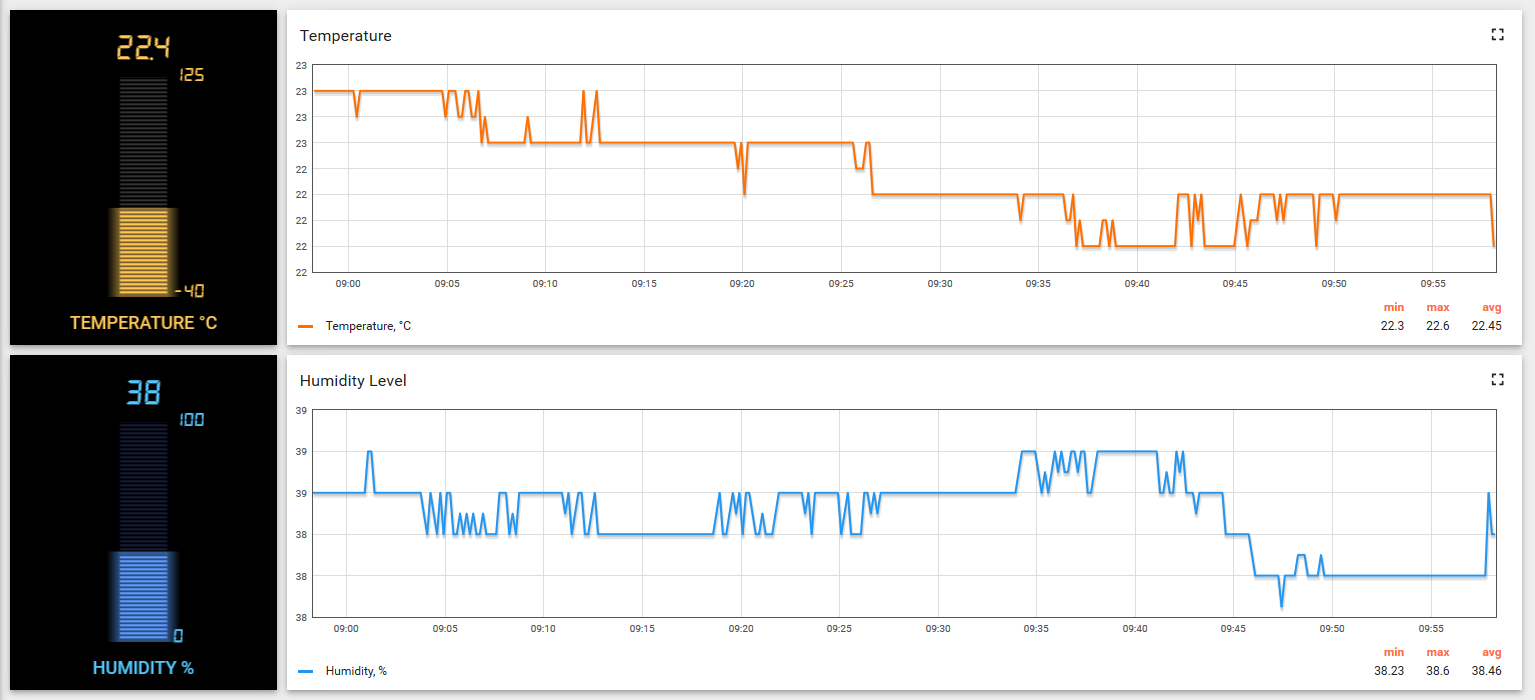
\includegraphics[width=\imageWidth\textwidth]{assets/thingsboard_dashboard.png}
    \caption{\label{fig:thingsboard_dashboard} ThingsBoard dashboard showing temperature and humidity data.}
\end{figure}

\begin{listing}[H]
    \inputminted[
        fontsize=\footnotesize,
        tabsize=2,
        breaklines,
        firstline=56,
        lastline=56]
        {python}
        {../rpi-coap/rpi-coap.py}
    \inputminted[
        fontsize=\footnotesize,
        tabsize=2,
        breaklines,
        firstline=64,
        lastline=69]
        {python}
        {../rpi-coap/rpi-coap.py}
    \caption{Method for getting data from DHT22 sensor.}
    \label{lst:get_data}
\end{listing}

\begin{listing}[H]
    \inputminted[
        tabsize=2,
        fontsize=\footnotesize,
        breaklines,
        firstline=90,
        lastline=90]
        {python}
        {../rpi-coap/rpi-coap.py}
    \inputminted[
        tabsize=2,
        fontsize=\footnotesize,
        breaklines,
        firstline=96,
        lastline=101]
        {python}
        {../rpi-coap/rpi-coap.py}
    \caption{Method for sending formatted data to the cloud.}
    \label{lst:send_data}
\end{listing}

Once the ThingsBoard cloud receives the data, the data is processed through the
ThingsBoard cloud's rules engine. For this study, no extra rules have been 
applied to the data handling. The default handling of data sent to the telemetry
endpoint is to identify the device that is sending the data, store the values
and update any dashboards associated with that device. The device is 
identified by the device access token sent as part of the request. An image 
of the ThingsBoard dashboard for this study is shown in 
\figref{fig:thingsboard_dashboard}. These dashboards are customisable and allow
for the data to be shown in realtime or show a selection of historical results.
The dashboard in \figref{fig:thingsboard_dashboard} has four display widgets:
one showing the last temperature reading, one showing all the latest temperature
readings for the previous hour, one showing the last humidity reading and one
showing all humidity readings in the last hour.
